% Generated by scripts/paper_figures.py from frozen files. Do not edit by hand.
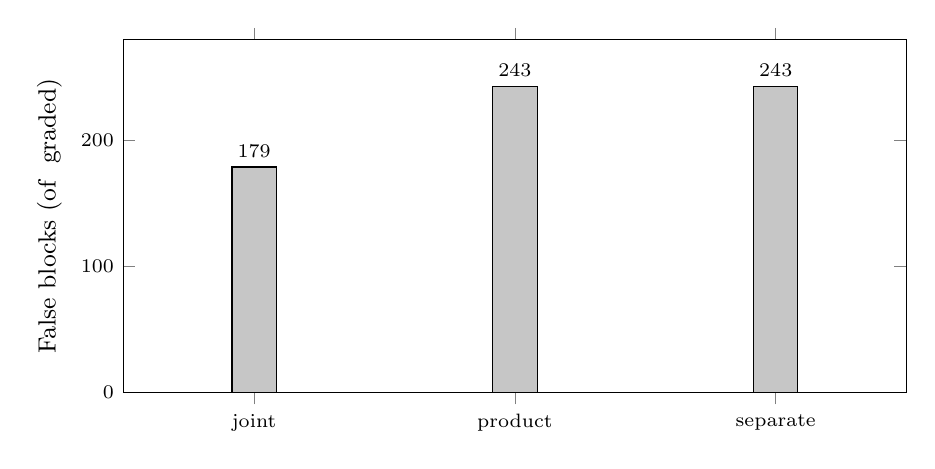
\begin{tikzpicture}
  \begin{axis}[ybar, width=0.95\columnwidth, height=0.5\columnwidth, bar width=16pt,
    symbolic x coords={joint,product,separate}, xtick=data, ymin=0, ymax=280,
    ylabel={False blocks (of \nQtwoGraded{} graded)}, nodes near coords,
    nodes near coords style={font=\scriptsize}, tick label style={font=\scriptsize},
    label style={font=\small}, enlarge x limits=0.25]
    \addplot[fill=gray!45] coordinates {(joint,179) (product,243) (separate,243)};
  \end{axis}
\end{tikzpicture}
